\documentclass[12pt]{article}

\setlength{\parindent}{0pt}  % No indent
\setlength{\parskip}{1em}    % Extra space between paragraphs

% Packages
\usepackage{amsmath, amssymb, graphicx, caption, subcaption, geometry}
\geometry{margin=1in}
\usepackage{fancyhdr}
\pagestyle{fancy}
\usepackage{hyperref}

% \lhead{Gaussian Process Lab}
% \rhead{Your Name}

% Title
\title{\textbf{Gaussian Process Regression for F1TENTH Vehicle Dynamics Lab Documentation}}
% \author{Your Name \\ Department of Electrical Engineering \\ Your University}
\date{\today}

\begin{document}

\maketitle

\begin{abstract}

This experiment investigates the application of Gaussian Process Regression (GPR) for modeling unknown functions from noisy data. We explore the theoretical foundations of GPs, implement them using Python and GPyTorch, and evaluate their performance on both synthetic and simulated datasets. The results highlight the strengths and limitations of GPR in capturing complex dynamics and providing uncertainty estimates.

\end{abstract}

\section{Introduction}
Gaussian Processes (GPs) provide a non-parametric Bayesian approach to regression problems. Unlike traditional regression, GPs yield not only point estimates but also confidence intervals, making them powerful for modeling uncertainty.

\section{Theory}

\subsection{Gaussian Processes}

A Gaussian Process is defined as a collection of random variables, any finite number of which have a joint Gaussian distribution. A GP is fully specified by its mean function $m(\mathbf{x})$ and covariance function $k(\mathbf{x}, \mathbf{x}')$:
\[
    f(\mathbf{x}) \sim \mathcal{GP}(m(\mathbf{x}), k(\mathbf{x}, \mathbf{x}'))
\]
Given training data $\mathcal{D} = \{\mathbf{X}, \mathbf{y}\}$ and a test point $\mathbf{x}_*$, the posterior predictive distribution is:
\[
    \mu_* = \mathbf{k}_*^\top(\mathbf{K} + \sigma_n^2 \mathbf{I})^{-1}\mathbf{y}, \quad
    \sigma_*^2 = k(\mathbf{x}_*, \mathbf{x}_*) - \mathbf{k}_*^\top(\mathbf{K} + \sigma_n^2 \mathbf{I})^{-1}\mathbf{k}_*
\]

\subsection{Vehicle Dynamics}

In the context of F1TENTH vehicles, the GP is used to model the relationship between state variables along with control input with the vehicle's dynamics. We may define the state transition as:
\[
    \mathbf{x}_{t+1} = f(\mathbf{z}_t) + \epsilon, \quad \epsilon \sim \mathcal{N}(0, \sigma_n^2)
\]
where $\mathbf{z}_t = \begin{bmatrix}\mathbf{x}_t & \mathbf{u}_t \end{bmatrix}^\top$ is the combined state and control input vector at time $t$.

For the state, we consider:
\[
    \mathbf{x} = \begin{bmatrix}
    \delta & v & \dot{\psi} & \beta
    \end{bmatrix}^\top
\]
where $\delta$ is the steering angle, $v$ is the velocity, $\dot{\psi}$ is the yaw rate, and $\beta$ is the slip angle.

And the control input is:
\[
    \mathbf{u} = \begin{bmatrix}
    u_1 & \delta
    \end{bmatrix}^\top
\]
where $u_1$ is the acceleration or speed command.

The dynamics function $f$ can be learned using GP regression, allowing us to predict future states given current states and control inputs. The dynamics can be obtained by differentiating the state variables with respect to time:
\[
    \mathbf{y} = {\mathbf{z}_{t+1} - \mathbf{z}_t \over \Delta t}
\]


\section{Experimental Setup}
\subsection{Data}
We use two datasets:
\begin{itemize}
    \item \textbf{Synthetic:} $y = \sin(x) + \epsilon$ with $\epsilon \sim \mathcal{N}(0, 0.1^2)$
    \item \textbf{Simulated:} F1TENTH vehicle dynamics simulation data from the Gym environment.
\end{itemize}

\subsubsection{Synthetic Data}

\begin{enumerate}
    \item To test the GP model basic functionality, the synthetic dataset consists of 1000 training points sampled uniformly from the interval $[0, 1]$. The corresponding outputs are generated using the sine function with added Gaussian noise. 
    \[
        y = \sin(x) + \epsilon, \quad \epsilon \sim \mathcal{N}(0, 0.1^2)
    \]

    \item To test the GP model's capability to detect and adapt to the change in the variation of the uncertainty, we also create a second synthetic dataset with heteroscedastic noise. In this dataset, the noise variance varies with the input value:
    \[
        y = \sin(x) + \epsilon, \quad \epsilon \sim \mathcal{N}(0, (0.1 + g(x))^2)
    \]
\end{enumerate}

\subsubsection{Simulated Data}

The simulated dataset is generated using the F1TENTH Gym environment. The vehicle is controlled using a simple policy, and state transitions are recorded over multiple episodes. The dataset includes state variables (steering angle, velocity, yaw rate, slip angle) and control inputs (speed, steering command).

The simple policy is defined as maintain a constant speed with a minor noise, and a steering command generated by summation of multiple sine waves with different frequencies and amplitudes to simulate a more complex driving behavior.




\subsection{Implementation}
The GP model is implemented using Python and the GPyTorch library. The code can be found in \href{https://github.com/SpectrumMu/f110-gp4dyn}{Git Repo}.

The implementation includes standard, sparse, and variational Gaussian Process  regression using a Radial Basis Function (RBF) kernel. A 6-to-1 GP model is first constructed and then extended to a 6-to-4 model for multi-output next-state prediction. Training is performed using the Adam optimizer with a learning rate of 0.1 for 100 epochs.


\section{Results and Discussion}
% \begin{figure}[h]
%     \centering
%     \includegraphics[width=0.6\textwidth]{gp_prediction.png}
%     \caption{GP prediction with confidence intervals on synthetic data}
%     \label{fig:gp_synthetic}
% \end{figure}

\begin{figure}[h]
    \centering
    \begin{subfigure}{0.45\textwidth}
        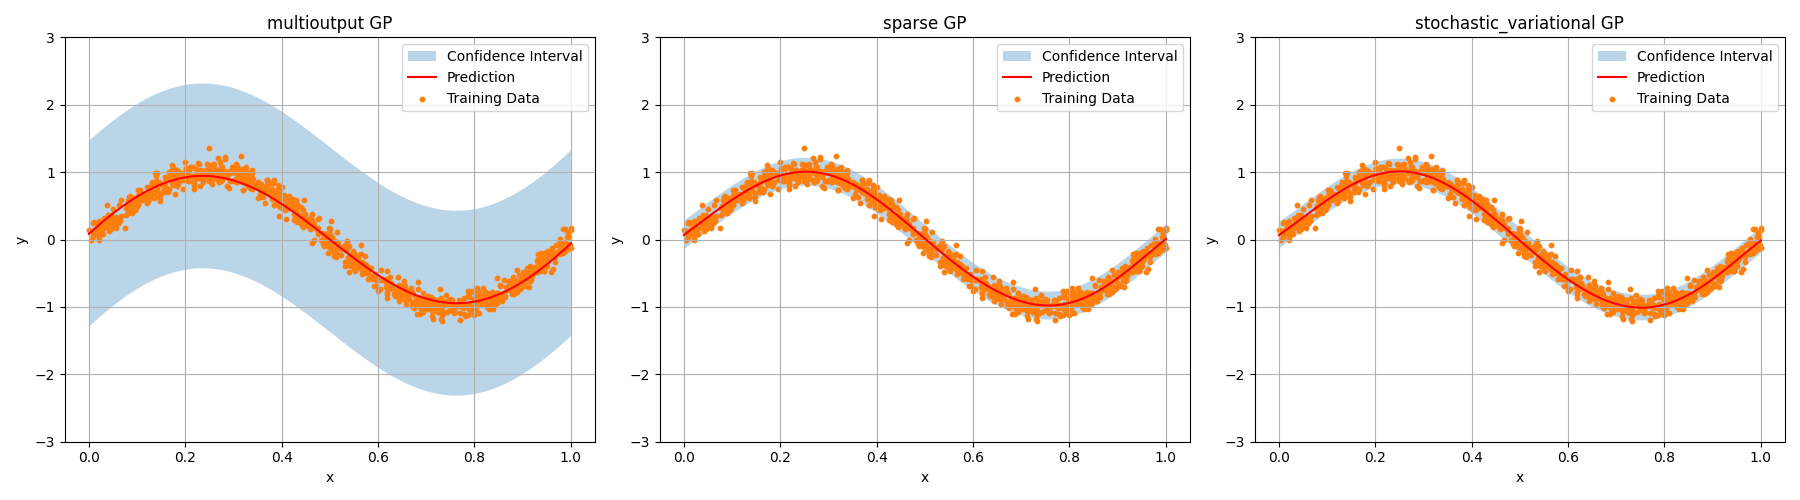
\includegraphics[width=\textwidth]{figs/data_1_fix.png}
        \caption{GP on Constant Std Synthetic Data}
        \label{fig:gp_synthetic_1}
    \end{subfigure}
    \hfill
    \begin{subfigure}{0.45\textwidth}
        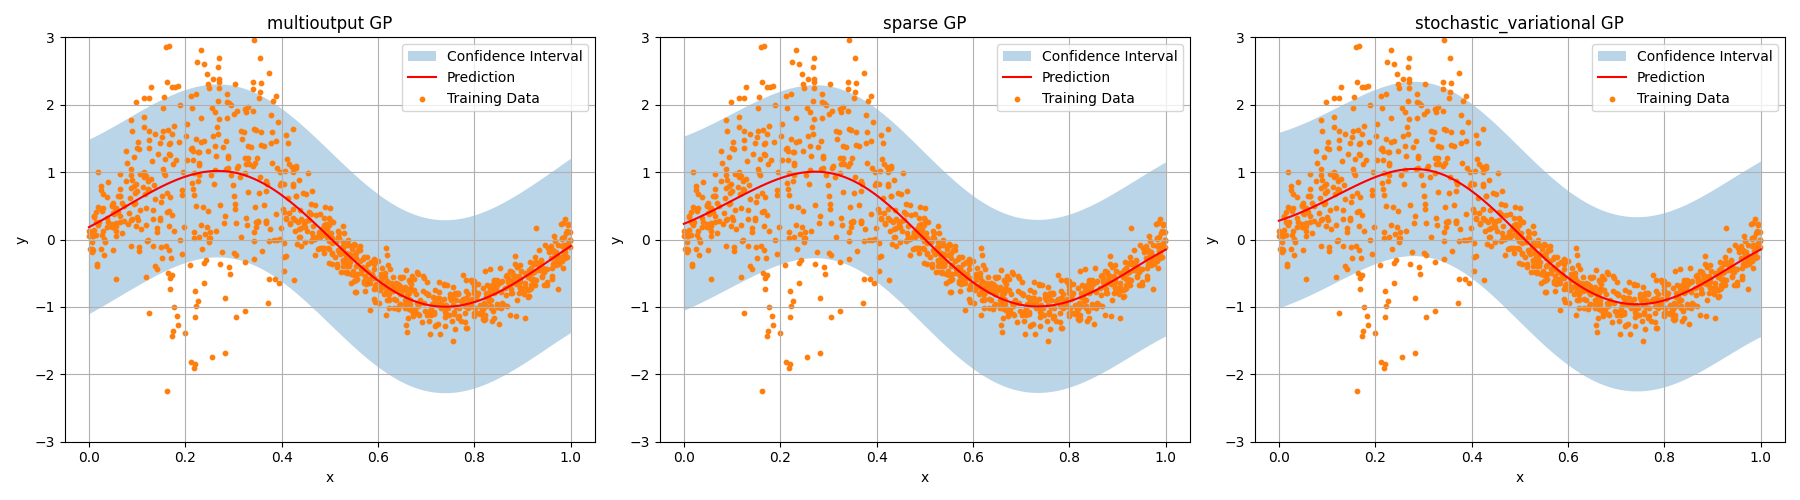
\includegraphics[width=\textwidth]{figs/data_1_vari.png}
        \caption{GP on Variational Std Synthetic Data}
        \label{fig:gp_synthetic_2}
    \end{subfigure}
    \caption{GP Regression on Synthetic Data}
    \label{fig:gp_results}
\end{figure}

The results of the GP regression on the synthetic datasets are shown in Figure \ref{fig:gp_results}. The GP model is able to capture the underlying function and provide uncertainty estimates, with constant uncertainty in Figure \ref{fig:gp_synthetic_1}. However, we observed that the GP model struggled to adapt to the varying uncertainty in Figure \ref{fig:gp_synthetic_2}, indicating a limitation in handling heteroscedastic noise.

\begin{figure}[h]
    \centering
    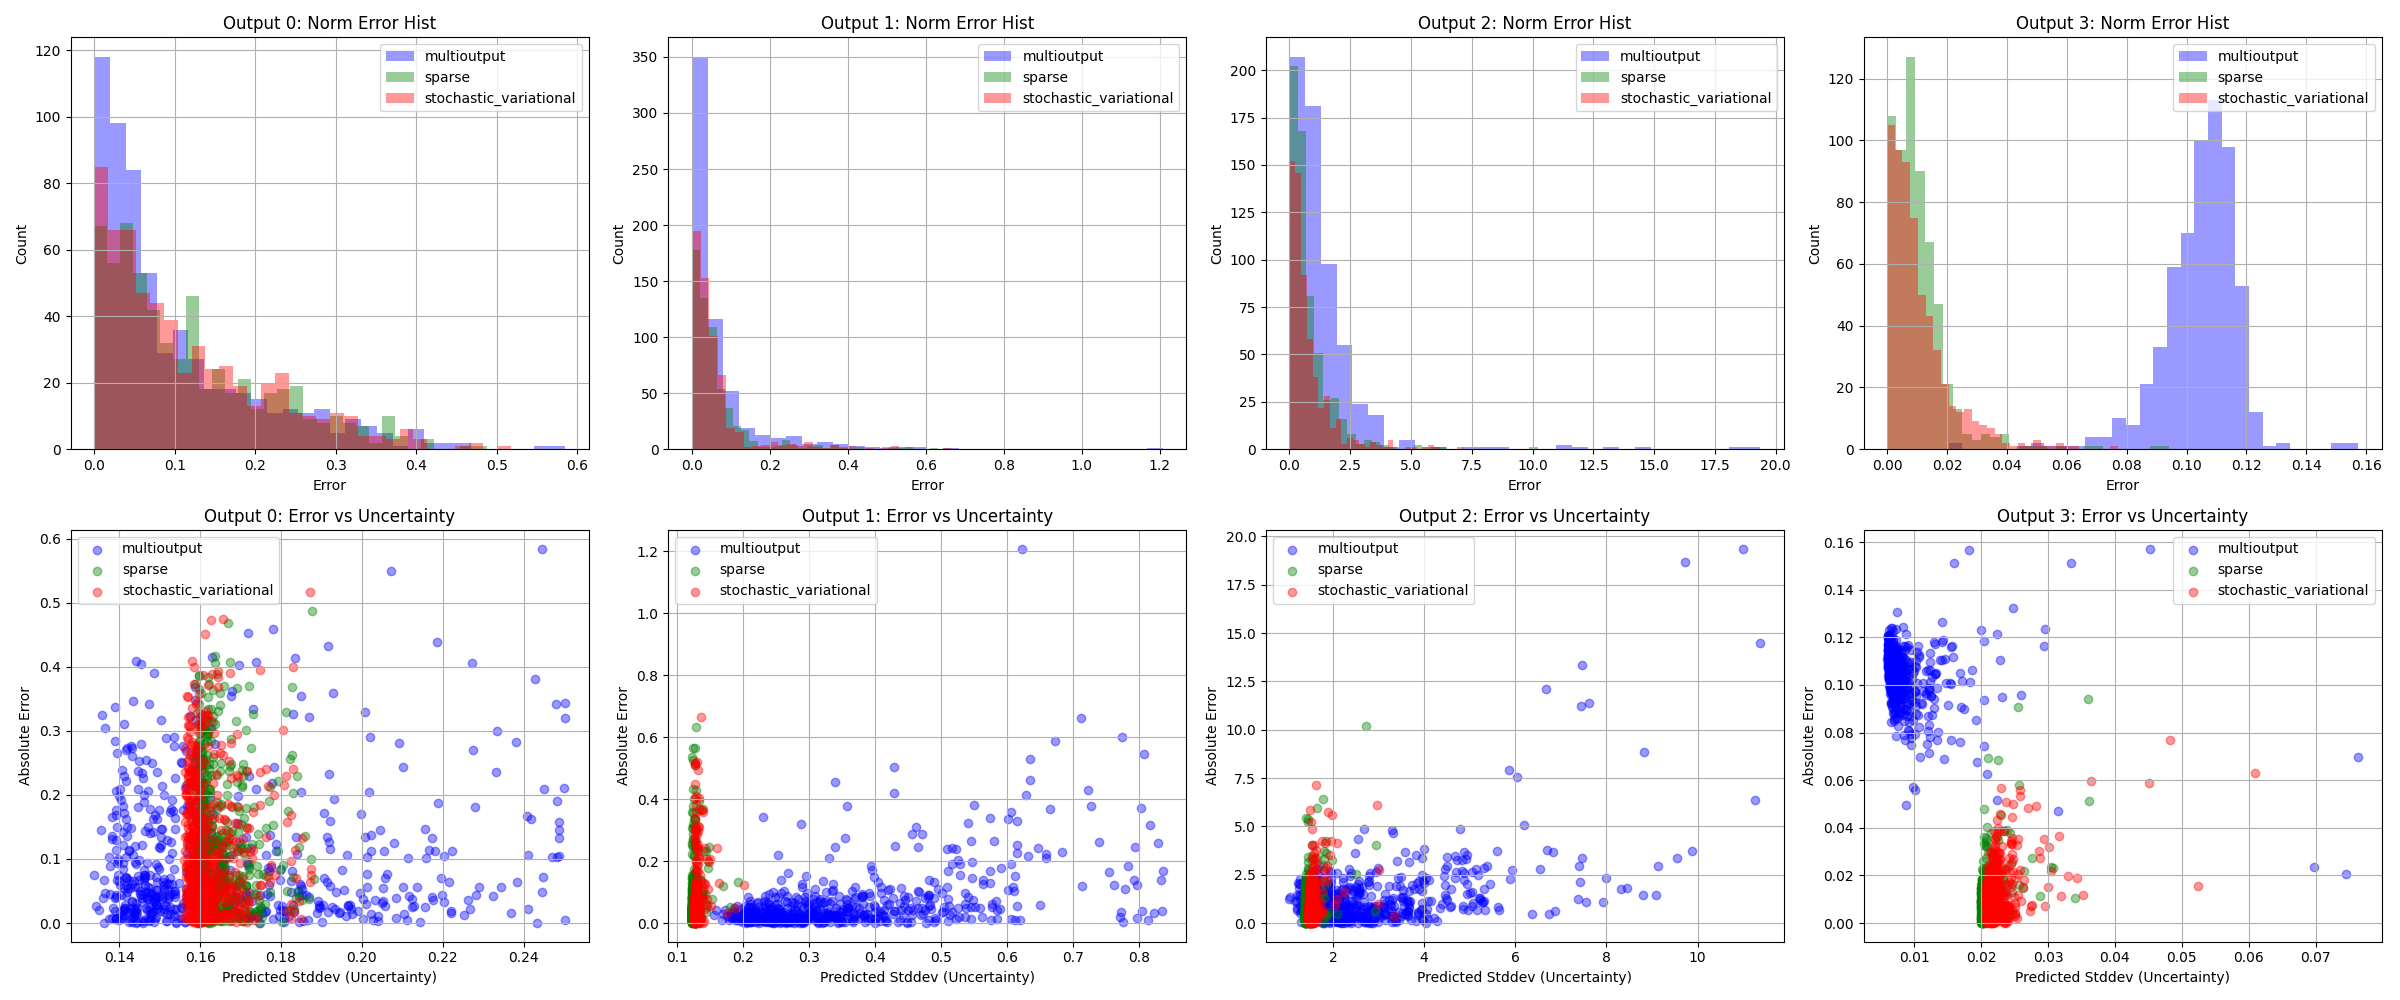
\includegraphics[width=0.9\textwidth]{figs/all_outputs_norm_hist_and_scatter_compare.png}
    \caption{GP Regression on Simulated F1TENTH Data}
    \label{fig:gp_simulated}
\end{figure}

The results on the simulated F1TENTH dataset, using all 3 GP models, are shown in Figure \ref{fig:gp_simulated}. The results indicate that the GP models cannot effectively capture the complex dynamics of the environment, leading to suboptimal performance. The error-uncertainty scatter plots show a weak correlation between prediction error and uncertainty, suggesting that the GP's uncertainty estimates may not be reliable in this context.

\section{Conclusion}
This experiment demonstrates the application of Gaussian Process Regression for modeling vehicle dynamics. While GPs provide valuable uncertainty estimates, their performance is limited in scenarios with heteroscedastic noise and complex dynamics. Future work could explore advanced GP models or hybrid approaches to improve predictive accuracy and uncertainty quantification.


\end{document}
